%% Generated by research/ablation/build_supplementary.py.
%% Do not hand-edit: change results/CLAIM_checklist.md (or the TRIPOD+AI table generator)
%% and re-run this script (hard rule 4).
\documentclass[10pt,a4paper]{article}
\usepackage[margin=2.2cm]{geometry}
\usepackage{booktabs}
\usepackage{longtable}
\usepackage{graphicx}
\usepackage[T1]{fontenc}
\usepackage{lmodern}
\usepackage[hidelinks]{hyperref}
\graphicspath{{figures/}}
\setlength{\parindent}{0pt}
\setlength{\parskip}{0.6em}
\renewcommand{\arraystretch}{1.25}

\title{Supplementary Material\\[0.3em]
\large Reporting checklists and case atlas}
\author{An Ablation-Grounded Ensemble for Dermoscopic Skin Lesion Classification:\\
Subgroup-Conditional Calibration, Abstention and Conformal Guarantees}
\date{}

\begin{document}
\maketitle

\section*{S1. CLAIM 2024 reporting checklist}


\textbf{CLAIM} --- Checklist for Artificial Intelligence in Medical Imaging. Originally Mongan, Moy \& Kahn Jr., \emph{Radiology: Artificial Intelligence} 2020;2(2):e200029 (an RSNA journal); this document follows the \textbf{2024 update}, Tejani et al., \emph{Radiology: Artificial Intelligence} 2024;6(4):e240300, which expands the checklist to \textbf{44 items}.


\textbf{On wording.} Item topics below are paraphrased in one line each. The authoritative wording is in the cited paper and is not reproduced here. This file records \emph{where in this project each item is addressed} and, where an item is not met, says so plainly rather than leaving it blank --- a checklist whose only function is to display ticks is worth nothing to a reviewer.


\textbf{Status vocabulary}


\begin{longtable}{@{}lp{0.75\textwidth}@{}}
\toprule
\textbf{Status} & \textbf{Meaning} \\
\midrule
\endfirsthead
\toprule
\textbf{Status} & \textbf{Meaning} \\
\midrule
\endhead
\bottomrule
\endfoot
\textbf{Met} & Addressed in the manuscript or a \texttt{results/} artifact, cited in the right-hand column. \\
\textbf{Partial} & Addressed, but with a stated limitation that a reviewer should see. \\
\textbf{Not met} & Not done. The reason is given. \\
\textbf{N/A} & Does not apply to a retrospective study on public datasets. \\
\end{longtable}


Generated for the manuscript in \texttt{paper/manuscript.tex}. Intended to be included as a supplementary appendix, not only as a repository file --- the point of a checklist is that a reviewer can read it.



\section*{Title and abstract}


\begin{longtable}{@{}rp{0.26\textwidth}lp{0.44\textwidth}@{}}
\toprule
\textbf{\#} & \textbf{Item} & \textbf{Status} & \textbf{Where} \\
\midrule
\endfirsthead
\toprule
\textbf{\#} & \textbf{Item} & \textbf{Status} & \textbf{Where} \\
\midrule
\endhead
\bottomrule
\endfoot
1 & Identifies the study as applying AI/ML to medical imaging & Met & Title; Abstract \\
2 & Structured abstract: aims, methods, results, conclusions & Met & Abstract (247 words) \\
\end{longtable}


\section*{Introduction}


\begin{longtable}{@{}rp{0.26\textwidth}lp{0.44\textwidth}@{}}
\toprule
\textbf{\#} & \textbf{Item} & \textbf{Status} & \textbf{Where} \\
\midrule
\endfirsthead
\toprule
\textbf{\#} & \textbf{Item} & \textbf{Status} & \textbf{Where} \\
\midrule
\endhead
\bottomrule
\endfoot
3 & Scientific and clinical background, including the intended use & Met & \S{}I Introduction \\
4 & Study objectives and hypotheses & Met & \S{}I, contributions list \\
\end{longtable}


\section*{Methods --- study design}


\begin{longtable}{@{}rp{0.26\textwidth}lp{0.44\textwidth}@{}}
\toprule
\textbf{\#} & \textbf{Item} & \textbf{Status} & \textbf{Where} \\
\midrule
\endfirsthead
\toprule
\textbf{\#} & \textbf{Item} & \textbf{Status} & \textbf{Where} \\
\midrule
\endhead
\bottomrule
\endfoot
5 & Prospective or retrospective study & Met & Retrospective, stated in \S{}III-A \\
6 & Study goal (model creation, exploratory, feasibility, non-inferiority) & Met & \S{}I --- model development and evaluation, explicitly not a clinical trial \\
7 & Ethical approval / institutional review & N/A & Public de-identified datasets (HAM10000, PAD-UFES-20); no new human-subject data collected. Stated in \S{}III-A \\
8 & Registration of the study protocol & \textbf{Not met} & Not registered. A pre-registered analysis plan is used instead: \texttt{results/analysis\_plan.json}, frozen before the single test read (S9) and hashed into \texttt{results/frozen\_artifacts.json} \\
9 & Sources of funding and role of funder & Met & Acknowledgements (\texttt{TODO} marker pending) \\
\end{longtable}


\section*{Methods --- data}


\begin{longtable}{@{}rp{0.26\textwidth}lp{0.44\textwidth}@{}}
\toprule
\textbf{\#} & \textbf{Item} & \textbf{Status} & \textbf{Where} \\
\midrule
\endfirsthead
\toprule
\textbf{\#} & \textbf{Item} & \textbf{Status} & \textbf{Where} \\
\midrule
\endhead
\bottomrule
\endfoot
10 & Data sources & Met & \S{}III-A; HAM10000 (Tschandl et al.), PAD-UFES-20 (Pacheco et al.) \\
11 & Eligibility criteria: how, by whom, and when data were selected & Met & \S{}III-A; \texttt{ml/preprocessing/split\_dataset.py} \\
12 & Data pre-processing steps & Met & \S{}III \emph{Backbones and training}; \texttt{ml/preprocessing/transforms.py}. Colour constancy was planned and \textbf{not} implemented --- reported as absent rather than omitted (Limitations) \\
13 & Selection of data subsets, if applicable & Met & \S{}III-A \\
14 & Definitions of data elements, with references to Common Data Elements & Partial & Class definitions in Table I. No formal CDE mapping --- dermoscopy has no widely adopted CDE set for these seven diagnoses \\
15 & De-identification methods & Met & Inherited from the source datasets, both released de-identified; stated in \S{}III-A \\
16 & How missing data were handled & Met & Missing \texttt{age}/\texttt{sex} are kept as an explicit \texttt{unknown} level and never folded into a real group --- \texttt{research/selective/fairness.py:load\_attributes}; the excluded counts are footnoted in Table IV \\
\end{longtable}


\section*{Methods --- ground truth}


\begin{longtable}{@{}rp{0.26\textwidth}lp{0.44\textwidth}@{}}
\toprule
\textbf{\#} & \textbf{Item} & \textbf{Status} & \textbf{Where} \\
\midrule
\endfirsthead
\toprule
\textbf{\#} & \textbf{Item} & \textbf{Status} & \textbf{Where} \\
\midrule
\endhead
\bottomrule
\endfoot
17 & Definition of the reference standard & Met & \S{}III-A; histopathology, follow-up, expert consensus or in-vivo confocal microscopy, per HAM10000's \texttt{dx\_type} \\
18 & Rationale for choosing the reference standard & Met & \S{}III-A \\
19 & Source of ground-truth annotations; qualifications of annotators & Met & \S{}III-A, deferred to the source dataset publications \\
20 & Annotation tools & N/A & Labels are dataset-supplied; no annotation performed in this work \\
21 & Measurement of inter- and intra-rater variability & \textbf{Not met} & Not available. The source datasets do not release per-rater labels, so variability cannot be computed here. Stated in Limitations \\
\end{longtable}


\section*{Methods --- data partitions}


\begin{longtable}{@{}rp{0.26\textwidth}lp{0.44\textwidth}@{}}
\toprule
\textbf{\#} & \textbf{Item} & \textbf{Status} & \textbf{Where} \\
\midrule
\endfirsthead
\toprule
\textbf{\#} & \textbf{Item} & \textbf{Status} & \textbf{Where} \\
\midrule
\endhead
\bottomrule
\endfoot
22 & Intended sample size and how it was determined & Partial & Fixed by the public datasets rather than powered in advance. Post-hoc power is reported where it binds: the under-40 subgroup gates in \texttt{research/stats/results\_oof/intersectional\_age\_sex.csv} and the conformal per-class certifiability counts \\
23 & How data were assigned to partitions; specify training, validation, test & Met & \S{}III-A; \textbf{all splits grouped by \texttt{lesion\_id}} with \texttt{assert\_no\_leakage()} enforced --- \texttt{ml/configs/splits/split\_v1.csv}, train 6,981 / val 1,532 / test 1,502 \\
24 & Level at which partitions are disjoint & Met & Lesion level, not image level. This is Hard Rule 1 of the project and the reason the bootstrap resamples lesions (\texttt{research/ablation/bootstrap.py}) \\
\end{longtable}


\section*{Methods --- model}


\begin{longtable}{@{}rp{0.26\textwidth}lp{0.44\textwidth}@{}}
\toprule
\textbf{\#} & \textbf{Item} & \textbf{Status} & \textbf{Where} \\
\midrule
\endfirsthead
\toprule
\textbf{\#} & \textbf{Item} & \textbf{Status} & \textbf{Where} \\
\midrule
\endhead
\bottomrule
\endfoot
25 & Detailed description of the model & Met & \S{}III \emph{Backbones and training}, \emph{Ensembling}, \emph{Test-time augmentation and calibration}; six CNN backbones, soft-vote ensemble, 24-view TTA, Dirichlet calibration \\
26 & Software libraries, frameworks, and packages & Met & \S{}III \emph{Backbones and training}, closing paragraph; Python 3.12, PyTorch 2.11 (CUDA 12.8), \texttt{timm}, scikit-learn 1.5. Pinned environment in \texttt{pyproject.toml} \\
27 & Initialisation of model parameters & Met & \S{}III \emph{Backbones and training}; ImageNet-pretrained, two-stage schedule (3 frozen head epochs, then fine-tune) \\
\end{longtable}


\section*{Methods --- training}


\begin{longtable}{@{}rp{0.26\textwidth}lp{0.44\textwidth}@{}}
\toprule
\textbf{\#} & \textbf{Item} & \textbf{Status} & \textbf{Where} \\
\midrule
\endfirsthead
\toprule
\textbf{\#} & \textbf{Item} & \textbf{Status} & \textbf{Where} \\
\midrule
\endhead
\bottomrule
\endfoot
28 & Details of training approach & Met & \S{}III \emph{Backbones and training}; \texttt{ml/configs/training\_config.yaml}, effective-number class weighting (Cui et al. 2019), seed 42 \\
29 & Method of selecting the final model & Met & \textbf{Macro-F1 on validation, never accuracy} (Hard Rule 3 --- 67\% \texttt{nv} makes accuracy meaningless). The one place this discipline was nearly broken is documented as a counter-example: ridge stacking has the best test and the worst val, and is therefore \emph{not} reported \\
30 & Ensembling techniques, if used & Met & \S{}III \emph{Ensembling}; uniform soft-vote over six CNNs. Rank-averaging, Nelder--Mead weights, ridge stacking and Caruana greedy selection were all evaluated and are reported as rejected \\
\end{longtable}


\section*{Methods --- evaluation}


\begin{longtable}{@{}rp{0.26\textwidth}lp{0.44\textwidth}@{}}
\toprule
\textbf{\#} & \textbf{Item} & \textbf{Status} & \textbf{Where} \\
\midrule
\endfirsthead
\toprule
\textbf{\#} & \textbf{Item} & \textbf{Status} & \textbf{Where} \\
\midrule
\endhead
\bottomrule
\endfoot
31 & Metrics of model performance, and why they were chosen & Met & \S{}III \emph{Metrics}; Macro-F1, balanced accuracy, escalation sensitivity, ECE, and the two clinical-utility definitions (Number Needed to Biopsy at a stated reference prevalence, False Reassurance Rate). Accuracy is explicitly excluded as a selection criterion \\
32 & Statistical measures of significance and uncertainty & Met & Lesion-grouped bootstrap for Macro-F1/ECE/AUC; \textbf{exact Clopper--Pearson for subgroup proportions} --- the switch rule is stated once in \texttt{research/stats/intervals.py} and applied by \texttt{research/run\_session7\_stats.py}. McNemar and DeLong with Holm--Bonferroni \\
33 & Robustness or sensitivity analysis & Met & 11-rung ablation ladder (\texttt{results/ablation\_table.csv}) plus five further combination levers reported as negative, two of them pre-registered rungs read in the single test pass (\texttt{results/session9/new\_rung\_comparisons.json}); $\lambda$ stability under lesion resampling, \texttt{research/agerule/results\_oof/}; NNB reported across a stated prevalence range 0.01--0.05 \\
34 & Methods for explainability or interpretability & Partial & Grad-CAM overlays (\texttt{paper/figures/gradcam/}, Fig. 7) plus a quantitative lesion-interior attribution fraction over the whole test split against Tschandl's segmentation masks (0.523 [0.509, 0.536], concentration ratio 3.45; \texttt{results/session9/attribution\_summary\_test.json}). Deliberately \textbf{not} claimed as causal evidence: for a misclassified case the map is taken w.r.t. the predicted class and lands on the lesion almost by construction, and Grad-CAM fails known sanity checks (Adebayo et al. 2018). The mechanistic claim rests on escalation-mass AUC instead \\
35 & Validation or testing on external data & Partial & Performed, on a \textbf{different modality}. The frozen system was applied unmodified to all 2,106 PAD-UFES-20 smartphone clinical images (\texttt{research/xdomain/results/}, \S{}IV \emph{External evaluation}): the six-CNN soft-vote reaches Macro-F1 0.167, below its own best member (0.188), and the frozen calibration map degrades it further to 0.133. This is a dataset-shift benchmark rather than external validation of the intended use; \textbf{no independent same-modality dermoscopy cohort has been evaluated}, and that gap is stated in Limitations \\
36 & Pre-specification of the analysis, and any deviations & Met & \texttt{results/analysis\_plan.json} (frozen before the single test read) and \texttt{results/comparison\_families.json} (every comparison family declared before its members are run, with confirmatory and exploratory sets separated) \\
\end{longtable}


\section*{Results}


\begin{longtable}{@{}rp{0.26\textwidth}lp{0.44\textwidth}@{}}
\toprule
\textbf{\#} & \textbf{Item} & \textbf{Status} & \textbf{Where} \\
\midrule
\endfirsthead
\toprule
\textbf{\#} & \textbf{Item} & \textbf{Status} & \textbf{Where} \\
\midrule
\endhead
\bottomrule
\endfoot
37 & Flow of participants or cases (a diagram is recommended) & Partial & Counts given in Table I and \S{}III-A; no CONSORT-style flow diagram. Nothing is excluded after ingestion, so the flow is a single step \\
38 & Demographic and clinical characteristics of each partition & Partial & Age band and sex reported, including the training escalating-class prior by band (\texttt{results/age\_band\_prior.csv}, 4.9\% under 40 vs 35.5\% at 60+) and an age $\times$ sex intersectional slice with its suppressed cells named. \textbf{Skin tone is unavailable for the development cohort}: HAM10000 ships no Fitzpatrick labels and the ITA image proxy is documented as invalid on dermoscopy. It is reported for the external cohort, where 1,302 of 2,106 images carry a Fitzpatrick label --- types I--IV are powered, V and VI are suppressed, so the analysis says nothing about darker skin \\
39 & Performance metrics for all partitions & Met & \texttt{results/ablation\_table.csv}; validation and OOF in \texttt{research/stats/results\_oof/} \\
40 & Estimates of diagnostic accuracy and their precision & Met & Every reported proportion carries a 95\% interval with its method named --- Table IV, \texttt{research/stats/results\_oof/age\_gap\_intervals.csv} \\
41 & Failure analysis of incorrectly classified cases & Met & \S{}V \emph{Confidently wrong is a distinct failure mode}; the under-40 blind spot, and specifically that it is a \emph{confidently}-wrong failure --- the abstention gate defers only 6.2\% of that band against 17.3\% at 60+, and rescues 11.1\% [0.014, 0.347] of its misses against 36.2\% [0.227, 0.515] at 60+. Across the split only 21 of 78 missed escalating lesions are deferred (\texttt{results/session9/orthogonality\_test.csv}) \\
\end{longtable}


\section*{Discussion}


\begin{longtable}{@{}rp{0.26\textwidth}lp{0.44\textwidth}@{}}
\toprule
\textbf{\#} & \textbf{Item} & \textbf{Status} & \textbf{Where} \\
\midrule
\endfirsthead
\toprule
\textbf{\#} & \textbf{Item} & \textbf{Status} & \textbf{Where} \\
\midrule
\endhead
\bottomrule
\endfoot
42 & Study limitations, including potential bias, statistical uncertainty, and generalisability & Met & \S{}VI Limitations; per-band calibration disparity, the intersectional suppressed cells, the stacking mismatch, the forfeited conformal guarantee under out-of-fold calibration, and the failure of the age rule to be orthogonal to abstention in the very band it targets are all named rather than omitted \\
43 & Implications for practice, including the intended use and clinical role & Met & \S{}V \emph{Clinical positioning}; framed around deployability --- decision rule, abstention, conformal sets and number-needed-to-biopsy rather than headline accuracy \\
\end{longtable}


\section*{Other information}


\begin{longtable}{@{}rp{0.26\textwidth}lp{0.44\textwidth}@{}}
\toprule
\textbf{\#} & \textbf{Item} & \textbf{Status} & \textbf{Where} \\
\midrule
\endfirsthead
\toprule
\textbf{\#} & \textbf{Item} & \textbf{Status} & \textbf{Where} \\
\midrule
\endhead
\bottomrule
\endfoot
44 & Registration number and name of registry; where the full protocol can be accessed; sources of funding & Partial & Not registered (item 8). Protocol, code and frozen artifact hashes are in the repository (\texttt{results/frozen\_artifacts.json}, \texttt{results/analysis\_plan.json}); repository URL is a \texttt{TODO} marker in the manuscript pending release \\
\end{longtable}



\section*{Summary}


\begin{longtable}{@{}lp{0.75\textwidth}@{}}
\toprule
\textbf{Status} & \textbf{Count} \\
\midrule
\endfirsthead
\toprule
\textbf{Status} & \textbf{Count} \\
\midrule
\endhead
\bottomrule
\endfoot
Met & 33 \\
Partial & 7 \\
Not met & 2 \\
N/A & 2 \\
\textbf{Total} & \textbf{44} \\
\end{longtable}


The 2 unmet items are honest gaps, not oversights, and both are stated in the manuscript: \textbf{no study registration} (mitigated by a frozen, hashed analysis plan) and \textbf{no inter-rater variability} (not derivable from the public label sets). Item 44 is partial for the same reason as item 8.


Item 35 moved from \emph{Not met} to \emph{Partial} once the external evaluation ran: it is a genuine external evaluation, but on smartphone clinical photography rather than an independent dermoscopy cohort, so it tests robustness under domain shift rather than validating the intended use. Calling it \emph{Met} would overstate what was done.


Section pointers here name subsections rather than letters, because subsection letters shift whenever the manuscript gains a section and silently rot.


\clearpage
\section*{S2. TRIPOD+AI (2024) cross-walk}

The cross-walk below is given in Table~\ref{tab:tripod_ai} and covers the $23$ reporting
domains of TRIPOD+AI, the standard for prediction models developed or validated with
artificial intelligence. It is reported here rather than in the main text because every item
resolves to a section of the manuscript or to a named artifact, and the table is a pointer
index rather than a result. Several rows point at tables that appear in the main manuscript
rather than in this standalone document; they are reproduced below (Table~\ref{tab:agegap},
Table~\ref{tab:external_battery}, Table~\ref{tab:external_safety}) so that this file is
readable on its own.

\begin{table*}[t]
\caption{TRIPOD+AI (2024) Reporting Checklist Cross-Walk: External Validation and Model Transportability}
\label{tab:tripod_ai}
\centering
\scriptsize
\begin{tabular}{lp{5.5cm}p{6.0cm}l}
\toprule
\textbf{Item} & \textbf{TRIPOD+AI Reporting Standard} & \textbf{Study Implementation in Manuscript} & \textbf{Manuscript Section / Artifact} \\
\midrule
1 & Identify study as developing/validating an AI model & Stated in Title and Abstract as clinical safety-net engineering & Title, Abstract \\
2 & Structured summary of objectives, data, validation & Comprehensive summary of multi-center findings and safety nets & Abstract \\
3a & Scientific rationale and clinical problem & Young-patient melanoma triage failure and age prior skew & Section~I \\
3b & Specific study aims and validation objectives & Formal hypothesis: argmax decision failure vs. information failure & Section~I, Section~II \\
4a & Study design and cohort origins & Multi-center: Vienna/Queensland (HAM), Barcelona (BCN), NY (MSK), Brazil (PAD) & Section~III-A, Section~V-F \\
4b & Setting and eligibility criteria & Lesion deduplication, age availability, SCC exclusion documented & Section~III-A, Table~I \\
5a & Target clinical outcome definitions & 7-class dermatopathology ground truth + 3-tier actionability hierarchy & Section~III-B, Table~\ref{tab:external_battery}, panel~(C) \\
6a & Input predictors and image acquisitions & Polarized contact dermoscopy (HAM/BCN/MSK) and smartphone photos (PAD) & Section~III-A \\
7 & Sample size and power calculations & Gate 0 power check ($\ge 100$ under-40 escalating lesions in BCN; $N=115$) & Section~V-F, \texttt{power\_report.md} \\
8 & Missing data handling & Missing age excluded from age-sliced metrics; null lesion IDs grouped & Section~III-A, Rule 6 \\
9a & Architecture and model development & 6 ImageNet CNNs, effective-number loss, 2-stage transfer learning & Section~III-C \\
10a & Model specification and hyperparameter freeze & Pre-registered protocol, SHA-256 locked checkpoints, Dirichlet calibration & Section~III-D, \texttt{frozen\_artifacts.json} \\
10b & Post-processing and decision rules & Escalation-mass threshold $\lambda_{\mathrm{opt}}=0.2818$; Mondrian conformal prediction & Section~IV, Section~V-B \\
11 & In-distribution performance metrics & Macro-F1, Balanced Acc, Escalation AUC, point-FRR, set-FRR, NNB & Section~V-A, Table~II \\
12 & Stratified subgroup evaluation & Stratified by age ($<40$, $40$--$59$, $60+$) and sex with cluster CIs & Section~V-C, Table~\ref{tab:agegap} \\
13a & External validation cohort specification & Multi-center Level 1 (BCN-20000, MSKCC) and Level 2 (PAD-UFES-20) & Section~V-F, Section~V-G \\
13b & Zero-target tuning discipline & Zero parameter fitting on external cohorts; HAM-OOF parameters frozen & Section~V-F, Hard Rule 3 \\
14 & Prior shift decoupling & Decomposed Bayesian prior shift from optical shift using Saerens EM & Section~V-G, Table~\ref{tab:external_battery}, panel~(B) \\
15 & Clinical decision curve analysis & Net Benefit evaluated across clinical thresholds $p_t \in [0.05, 0.20]$ & Section~V-E, Table~\ref{tab:external_battery}, panel~(D) \\
16 & Algorithmic fairness assessment & Stratified by Fitzpatrick skin types I--IV; V/VI suppressed per power gates & Section~V-G, Table~\ref{tab:external_safety}, panel~(B) \\
17 & Shift detection and safety nets & Mahalanobis OOD distance ($\mathrm{AUROC}=0.9148$) and conformal set widening & Section~V-G, Table~\ref{tab:external_safety}, panel~(A) \\
18 & Risk of bias and data leakage & Strict lesion-grouped split verification (\texttt{assert\_no\_leakage()}) & Section~III-A \\
19 & Interpretation of mechanistic findings & Argmax fails due to prior skew, not feature representation failure & Section~VI-A \\
20 & Causal validation via comparison arm & \emph{Withdrawn.} The arm requires retraining on BCN+MSK; the published checkpoints are frozen, so it was never run. Entered into the Holm family at $p=1.0$ & Section~VI-C (Limitations) \\
21 & Clinical deployment implications & Two-tiered triage, local calibration requirement, visible uncertainty & Section~VI-B \\
22 & Study limitations & Conformal non-exchangeability, underpowered Fitzpatrick V/VI sample & Section~VI-C \\
23 & Reproducibility and open artifacts & Code, split manifests, scripts, and pre-registration hashes published & Section~VII, \texttt{post\_s11\_provenance.json} \\
\bottomrule
\end{tabular}
\vspace{1mm}
\parbox{\linewidth}{\raggedright \emph{Compliance}: Formal cross-walk of the 23 reporting domains of TRIPOD+AI (2024 update) for transparent reporting of artificial intelligence prediction models in healthcare.}
\end{table*}


\clearpage
\section*{S2a. Tables cited by the cross-walk}

% Generated by research/run_session7_stats.py -- do not hand-edit (hard rule 4).
% Test column filled by the S9 single pre-registered test pass.
\begin{table*}[t]
\centering
\caption{Escalation sensitivity by patient age band, with $95\%$ confidence intervals. Intervals marked CP are exact Clopper--Pearson; those marked boot are lesion-grouped percentile bootstrap. The exact interval leads wherever the numerator is small, because the percentile bootstrap cannot reach the upper tail at those counts and would understate the uncertainty. Validation and out-of-fold estimates are shown side by side: the OOF split carries substantially more escalating cases in the under-40 band, which is why the age-conditional rule is fitted there. The test column is reported once, from the single pre-registered pass of Session~9; it is scored by the same deployed system as the OOF column and is not a like-for-like replication of the validation column, which different models scored on different patients.}
\label{tab:agegap}
\begin{tabular}{lcccccc}
\toprule
& \multicolumn{2}{c}{Validation} & \multicolumn{2}{c}{OOF} & \multicolumn{2}{c}{Test} \\
\cmidrule(lr){2-3}\cmidrule(lr){4-5}\cmidrule(lr){6-7}
Age band & Sensitivity [95\% CI] & $k/n$ & Sensitivity [95\% CI] & $k/n$ & Sensitivity [95\% CI] & $k/n$ \\
\midrule
$<$40 & $0.545$ [0.322, 0.756]$^{\text{CP}}$ & $12/22$ & $0.547$ [0.382, 0.716]$^{\text{boot}}$ & $35/64$ & $0.143$ [0.030, 0.363]$^{\text{CP}}$ & $3/21$ \\
40-59 & $0.550$ [0.392, 0.714]$^{\text{boot}}$ & $33/60$ & $0.612$ [0.547, 0.674]$^{\text{boot}}$ & $243/397$ & $0.814$ [0.694, 0.918]$^{\text{boot}}$ & $57/70$ \\
60+ & $0.774$ [0.696, 0.838]$^{\text{boot}}$ & $175/226$ & $0.733$ [0.697, 0.768]$^{\text{boot}}$ & $655/893$ & $0.764$ [0.683, 0.836]$^{\text{boot}}$ & $152/199$ \\
All ages & $0.714$ [0.644, 0.783]$^{\text{boot}}$ & $220/308$ & $0.690$ [0.657, 0.721]$^{\text{boot}}$ & $935/1356$ & $0.731$ [0.665, 0.793]$^{\text{boot}}$ & $212/290$ \\
\bottomrule
\end{tabular}
\par\smallskip\footnotesize Patients with no recorded age are excluded from the bands above: $10$ validation images ($0$ escalating) and $38$ OOF images ($2$ escalating), and $9$ test images ($0$ escalating). They are retained in the All-ages row and in \texttt{age\_gap\_intervals.csv}.
\end{table*}


% generated by research/external/render_composite_tables.py -- do not hand-edit
% supersedes external_table_{bcn_age_replication,pad_prior_shift,cross_cohort_triage,
%   decision_curve,conformal_shift,fitzpatrick_slices}.tex, which stay on disk as the
%   per-analysis outputs of their own scripts but are no longer part of the manuscript.
\begin{table*}[t]
\centering
\caption{External validity battery. All four panels score the deployed system unmodified -- uniform six-CNN soft-vote, 24-view TTA, frozen HAM10000-OOF Dirichlet map (\texttt{selective/results\_oof/fit\_state.json}) and frozen per-band $\lambda$ ($<$40: $0.26$, 40--59: $0.74$, 60+: $0.33$) -- so no parameter in any row is fitted on the cohort it is evaluated on. Point estimates are image-level; intervals resample lesions, except proportions with fewer than 30 events, which take the exact Clopper--Pearson interval. Panel~(A): the pre-registered contingency fired --- Claim~A (a cohort-invariant escalation-mass AUC) fails, with a spread of 0.105 across centres, and the Claim~B ordering is reversed rather than non-monotonic, so the three point estimates are reported with intervals and no trend is fitted. The confirmatory member \texttt{E1\_under40\_sens\_frozen\_lambda\_vs\_argmax} (BCN-20000, exact McNemar over 27 discordant cases) gives $p = 1.49 \times 10^{-8}$, Holm upper bound over the five-member family $= 7.45 \times 10^{-8}$; because $\lambda \ge 0$ can only add escalating predictions the test is one-sided by construction and certifies that cases were rescued, not that the rule is net-beneficial --- that trade is the last two columns. MSKCC's label space holds only \textsc{nv}, \textsc{mel} and \textsc{bkl}, so seven-class Macro-F1 is undefined there. Panel~(B) confirmatory member \texttt{E2\_em\_macro\_f1\_vs\_raw} is significant in the \emph{wrong} direction ($\chi^2 = 98.73$, $p = 2.89 \times 10^{-23}$, 321 cases correct only without the correction against 113 only with it). Panel~(C) point-FRR is the fraction of malignant Tier-1 lesions predicted Tier~3; NNB is the number needed to biopsy at reference prevalence $\pi$. $^{\dagger}$Panel~(D)'s test column is reconstructed from the frozen Session~9 artifacts (\texttt{results/session9/agerule\_test.csv}: TP, FP and $N$ only) and involves no new read of the test split.}
\label{tab:external_battery}
\scriptsize
\setlength{\tabcolsep}{3.2pt}
\begin{tabular}{@{}lcccccccc@{}}
\toprule
\multicolumn{9}{@{}l}{\textbf{(A) Three-centre dose--response of the under-40 escalation failure (E1).} Centres ordered by ascending prior skew. No parameter is fitted on BCN-20000 or MSKCC.} \\
\addlinespace[0.2em]
Cohort & Skew & \multicolumn{3}{c}{Escalation-mass AUC by age band} & \multicolumn{4}{c}{Under-40 escalation sensitivity} \\
\cmidrule(lr){3-5}\cmidrule(l{0.4em}){6-9}
 & $60{+}/{<}40$ & $<$40 [95\% CI] & 40--59 & 60+ & argmax [95\% CI] & mel.\ only & frozen $\lambda$ & $\Delta$ referral \\
\midrule
BCN-20000 & 3.83$\times$ & 0.791 [0.726, 0.843] & 0.826 & 0.795 & 0.279 [0.179, 0.382] & 0.274 & \textbf{0.352} & +0.026 \\
MSKCC & 6.54$\times$ & 0.790 [0.703, 0.867] & 0.693 & 0.694 & 0.333 [0.186, 0.510] & 0.333 & \textbf{0.389} & +0.019 \\
HAM10000 (source) & 8.45$\times$ & 0.895 [0.837, 0.944] & 0.955 & 0.934 & 0.547 [0.391, 0.708] & 0.490 & \textbf{0.625} & +0.024 \\
\midrule
\multicolumn{9}{@{}l}{\textbf{(B) PAD-UFES-20 prior decoupling (E2).} All $N=2{,}106$ images, no weights retrained. \textsc{oracle} uses the true target prior and is a ceiling, not a deployable system.} \\
\addlinespace[0.2em]
Variant & Deployable & Macro-F1 & Bal.\ acc. & Accuracy & Esc.\ sens. & Mel.\ recall & Missed serious &  \\
\midrule
Raw soft-vote & yes & 0.1669 & 0.3097 & 0.2626 & 0.3565 & 0.1154 & 1{,}047 &  \\
Dirichlet (deployed) & yes & 0.1303 & 0.2931 & 0.2137 & 0.2207 & 0.1154 & 1{,}268 &  \\
EM prior (Saerens) & yes & 0.1018 & 0.1035 & 0.1638 & 0.4155 & 0.0000 & 951 &  \\
Oracle prior & \textsc{oracle} & 0.2534 & 0.3327 & 0.4435 & 0.8949 & 0.0577 & 171 &  \\
Dirichlet $\rightarrow$ EM & yes & 0.1239 & 0.3079 & 0.2203 & 0.1223 & 0.0000 & 1{,}428 &  \\
\midrule
\multicolumn{9}{@{}l}{\textbf{(C) Three-tier clinical actionability (E3).} Tier~1 urgent biopsy (\textsc{mel}, \textsc{bcc}, \textsc{scc}); Tier~2 consult (\textsc{akiec}); Tier~3 discharge.} \\
\addlinespace[0.2em]
Cohort / configuration & Tier acc. & T1 sens. & T1 spec. & point-FRR & Missed T1 & \multicolumn{3}{c}{NNB at $\pi = 0.01/0.03/0.05$} \\
\cmidrule(l{0.4em}){7-9}
\midrule
HAM10000 OOF, raw & 0.8936 & 0.6781 & 0.9509 & 0.2875 & 326 & 8.17 & 3.34 & 2.38 \\
HAM10000 OOF, calibrated & 0.8986 & 0.6578 & 0.9584 & 0.3289 & 373 & 7.25 & 3.04 & 2.20 \\
PAD-UFES-20, raw & 0.3732 & 0.2698 & 0.9446 & 0.5195 & 466 & 21.34 & 7.64 & 4.90 \\
PAD-UFES-20, calibrated & 0.3310 & 0.2185 & 0.9644 & 0.6756 & 606 & 17.11 & 6.26 & 4.09 \\
PAD-UFES-20, oracle prior & 0.4720 & 0.4771 & 0.7469 & 0.0524 & 47 & 53.51 & 18.15 & 11.08 \\
\midrule
\multicolumn{9}{@{}l}{\textbf{(D) Decision-curve net benefit of the frozen age rule (E6).} $\mathrm{NB} = \mathrm{TP}/N - (\mathrm{FP}/N)\,p_t/(1-p_t)$; $\Delta$ is $\lambda$-rule minus argmax under a lesion-grouped paired bootstrap, bold where the interval excludes zero.} \\
\addlinespace[0.2em]
$p_t$ & Biopsy all & Argmax & $\lambda$-rule & Risk model & $\Delta$ & 95\% CI & Test $\Delta^{\dagger}$ &  \\
\midrule
\multicolumn{9}{@{}l}{\textit{All ages}} \\
0.05 & 0.1518 & 0.1327 & 0.1589 & 0.1759 & \textbf{+0.0263} & [+0.0214, +0.0315] & +0.0156 &  \\
0.10 & 0.1047 & 0.1306 & 0.1534 & 0.1633 & \textbf{+0.0228} & [+0.0178, +0.0282] & +0.0114 &  \\
0.15 & 0.0520 & 0.1283 & 0.1472 & 0.1544 & \textbf{+0.0189} & [+0.0138, +0.0243] & +0.0067 &  \\
0.20 & -0.0072 & 0.1257 & 0.1403 & 0.1449 & \textbf{+0.0146} & [+0.0093, +0.0199] & +0.0015 &  \\
\multicolumn{9}{@{}l}{\textit{Age $<$40}} \\
0.05 & -0.0016 & 0.0253 & 0.0280 & 0.0280 & +0.0027 & [-0.0002, +0.0065] & +0.0053 &  \\
0.10 & -0.0572 & 0.0239 & 0.0254 & 0.0195 & +0.0015 & [-0.0015, +0.0053] & +0.0034 &  \\
0.15 & -0.1194 & 0.0224 & 0.0226 & 0.0144 & +0.0002 & [-0.0032, +0.0042] & +0.0014 &  \\
0.20 & -0.1893 & 0.0207 & 0.0193 & 0.0125 & -0.0013 & [-0.0053, +0.0029] & -0.0009 &  \\
\bottomrule
\end{tabular}
\end{table*}


% generated by research/external/render_composite_tables.py -- do not hand-edit
% supersedes external_table_{bcn_age_replication,pad_prior_shift,cross_cohort_triage,
%   decision_curve,conformal_shift,fitzpatrick_slices}.tex, which stay on disk as the
%   per-analysis outputs of their own scripts but are no longer part of the manuscript.
\begin{table*}[t]
\centering
\caption{Safety nets under distribution shift. Panel~(A): the shift is detectable and the conformal sets widen under it, converting silent point errors into visible uncertainty --- but coverage itself degrades sharply, and the guarantee does not survive the move. Split conformal finite-sample coverage guarantees hold under exchangeability. External cohorts (PAD-UFES-20) are by construction non-exchangeable; coverage is reported as an empirical audit of safety-net widening behavior. Panel~(B): across the 4 adequately powered strata the Tier-1 sensitivity spread is 0.067 and it is \emph{not} monotonic in Fitzpatrick type (I~0.269, II~0.203, III~0.203, IV~0.231), so these data do not reproduce the reported darker-skin penalty. Only 1{,}302 of the 2{,}106 lesions carry a Fitzpatrick label at all; the two darkest strata are suppressed at $n=8$ and $n=1$, so this cohort cannot speak to darker skin. The unlabelled remainder holds no Tier-1 lesion, so a pooled labelled-versus-unlabelled gap is a data-completeness artefact and is not reported here as a skin-tone effect.}
\label{tab:external_safety}
\footnotesize
\setlength{\tabcolsep}{4pt}
\begin{tabular}{@{}lcccccccc@{}}
\toprule
\multicolumn{9}{@{}l}{\textbf{(A) Shift detection and conformal set widening.} In-distribution reference is the HAM10000-OOF tuning half, held out from the quantile estimate; the shifted cohort is PAD-UFES-20.} \\
\addlinespace[0.2em]
\multicolumn{9}{@{}l}{\emph{Mahalanobis detector} (fit on HAM10000 train features, no refit): median score 485 in distribution against 8{,}717 under shift (18.0$\times$ separation), AUROC 0.9128.} \\
\addlinespace[0.3em]
Conformal method & \multicolumn{4}{c}{In distribution (HAM10000 OOF)} & \multicolumn{4}{c}{Under shift (PAD-UFES-20)} \\
\cmidrule(lr){2-5}\cmidrule(l{0.4em}){6-9}
 & Marginal & Serious & set-FRR & Mean $|\mathcal{C}|$ & Marginal & Serious & set-FRR & Mean $|\mathcal{C}|$ \\
\midrule
LAC marginal $\alpha=0.10$ & 0.9052 & 0.7192 & 0.2526 & 1.08 & 0.2379 & 0.1217 & 0.7462 & 1.15 \\
LAC Mondrian $\alpha=0.10$ & 0.8816 & 0.8990 & 0.0743 & 1.26 & 0.4136 & 0.3516 & 0.2747 & 2.10 \\
LAC Mondrian $\alpha=0.05$ & 0.9365 & 0.9406 & 0.0386 & 2.33 & 0.6220 & 0.5722 & 0.1057 & 3.37 \\
APS Mondrian $\alpha=0.05$ & 0.9465 & 0.9495 & 0.0297 & 2.49 & 0.6548 & 0.5907 & 0.0725 & 4.06 \\
\midrule
\multicolumn{9}{@{}l}{\textbf{(B) Fitzpatrick skin-tone strata (PAD-UFES-20).} Pre-registered reporting gates: $N \ge 30$ and $N_{\text{Tier 1}} \ge 10$. Intervals are exact Clopper--Pearson; conformal sets are Mondrian $\alpha=0.05$.} \\
\addlinespace[0.2em]
Stratum & $N$ & $N_{\text{Tier 1}}$ & Tier-1 sens.\ [95\% CI] & point-FRR & set-FRR [95\% CI] & Mean $|\mathcal{C}|$ &  &  \\
\midrule
Type I & 137 & 104 & 0.269 [0.187, 0.365] & 0.606 & 0.096 [0.047, 0.170] & 3.48 &  &  \\
Type II & 750 & 537 & 0.203 [0.170, 0.239] & 0.680 & 0.060 [0.041, 0.083] & 3.50 &  &  \\
Type III & 347 & 227 & 0.203 [0.152, 0.261] & 0.709 & 0.101 [0.065, 0.148] & 3.42 &  &  \\
Type IV & 59 & 26 & 0.231 [0.090, 0.436] & 0.615 & 0.077 [0.009, 0.251] & 3.00 &  &  \\
Type V & 8 & 3 & \multicolumn{3}{c}{\emph{suppressed: $N < 30$; $N_{\text{Tier 1}} < 10$}} & 3.38 &  &  \\
Type VI & 1 & 0 & \multicolumn{3}{c}{\emph{suppressed: $N < 30$; no Tier-1 lesion, so Tier-1 rates are undefined}} & 4.00 &  &  \\
Unlabelled / missing & 804 & 0 & \multicolumn{3}{c}{\emph{suppressed: no Tier-1 lesion, so Tier-1 rates are undefined}} & 3.31 &  &  \\
\bottomrule
\end{tabular}
\end{table*}


\clearpage
\section*{S3. Case atlas: lesions the age-conditional rule rescues}

Fig.~\ref{fig:case_atlas} shows exemplar lesions whose predicted class changes under the
frozen age-conditional rule.

\begin{figure}[h]
\centering
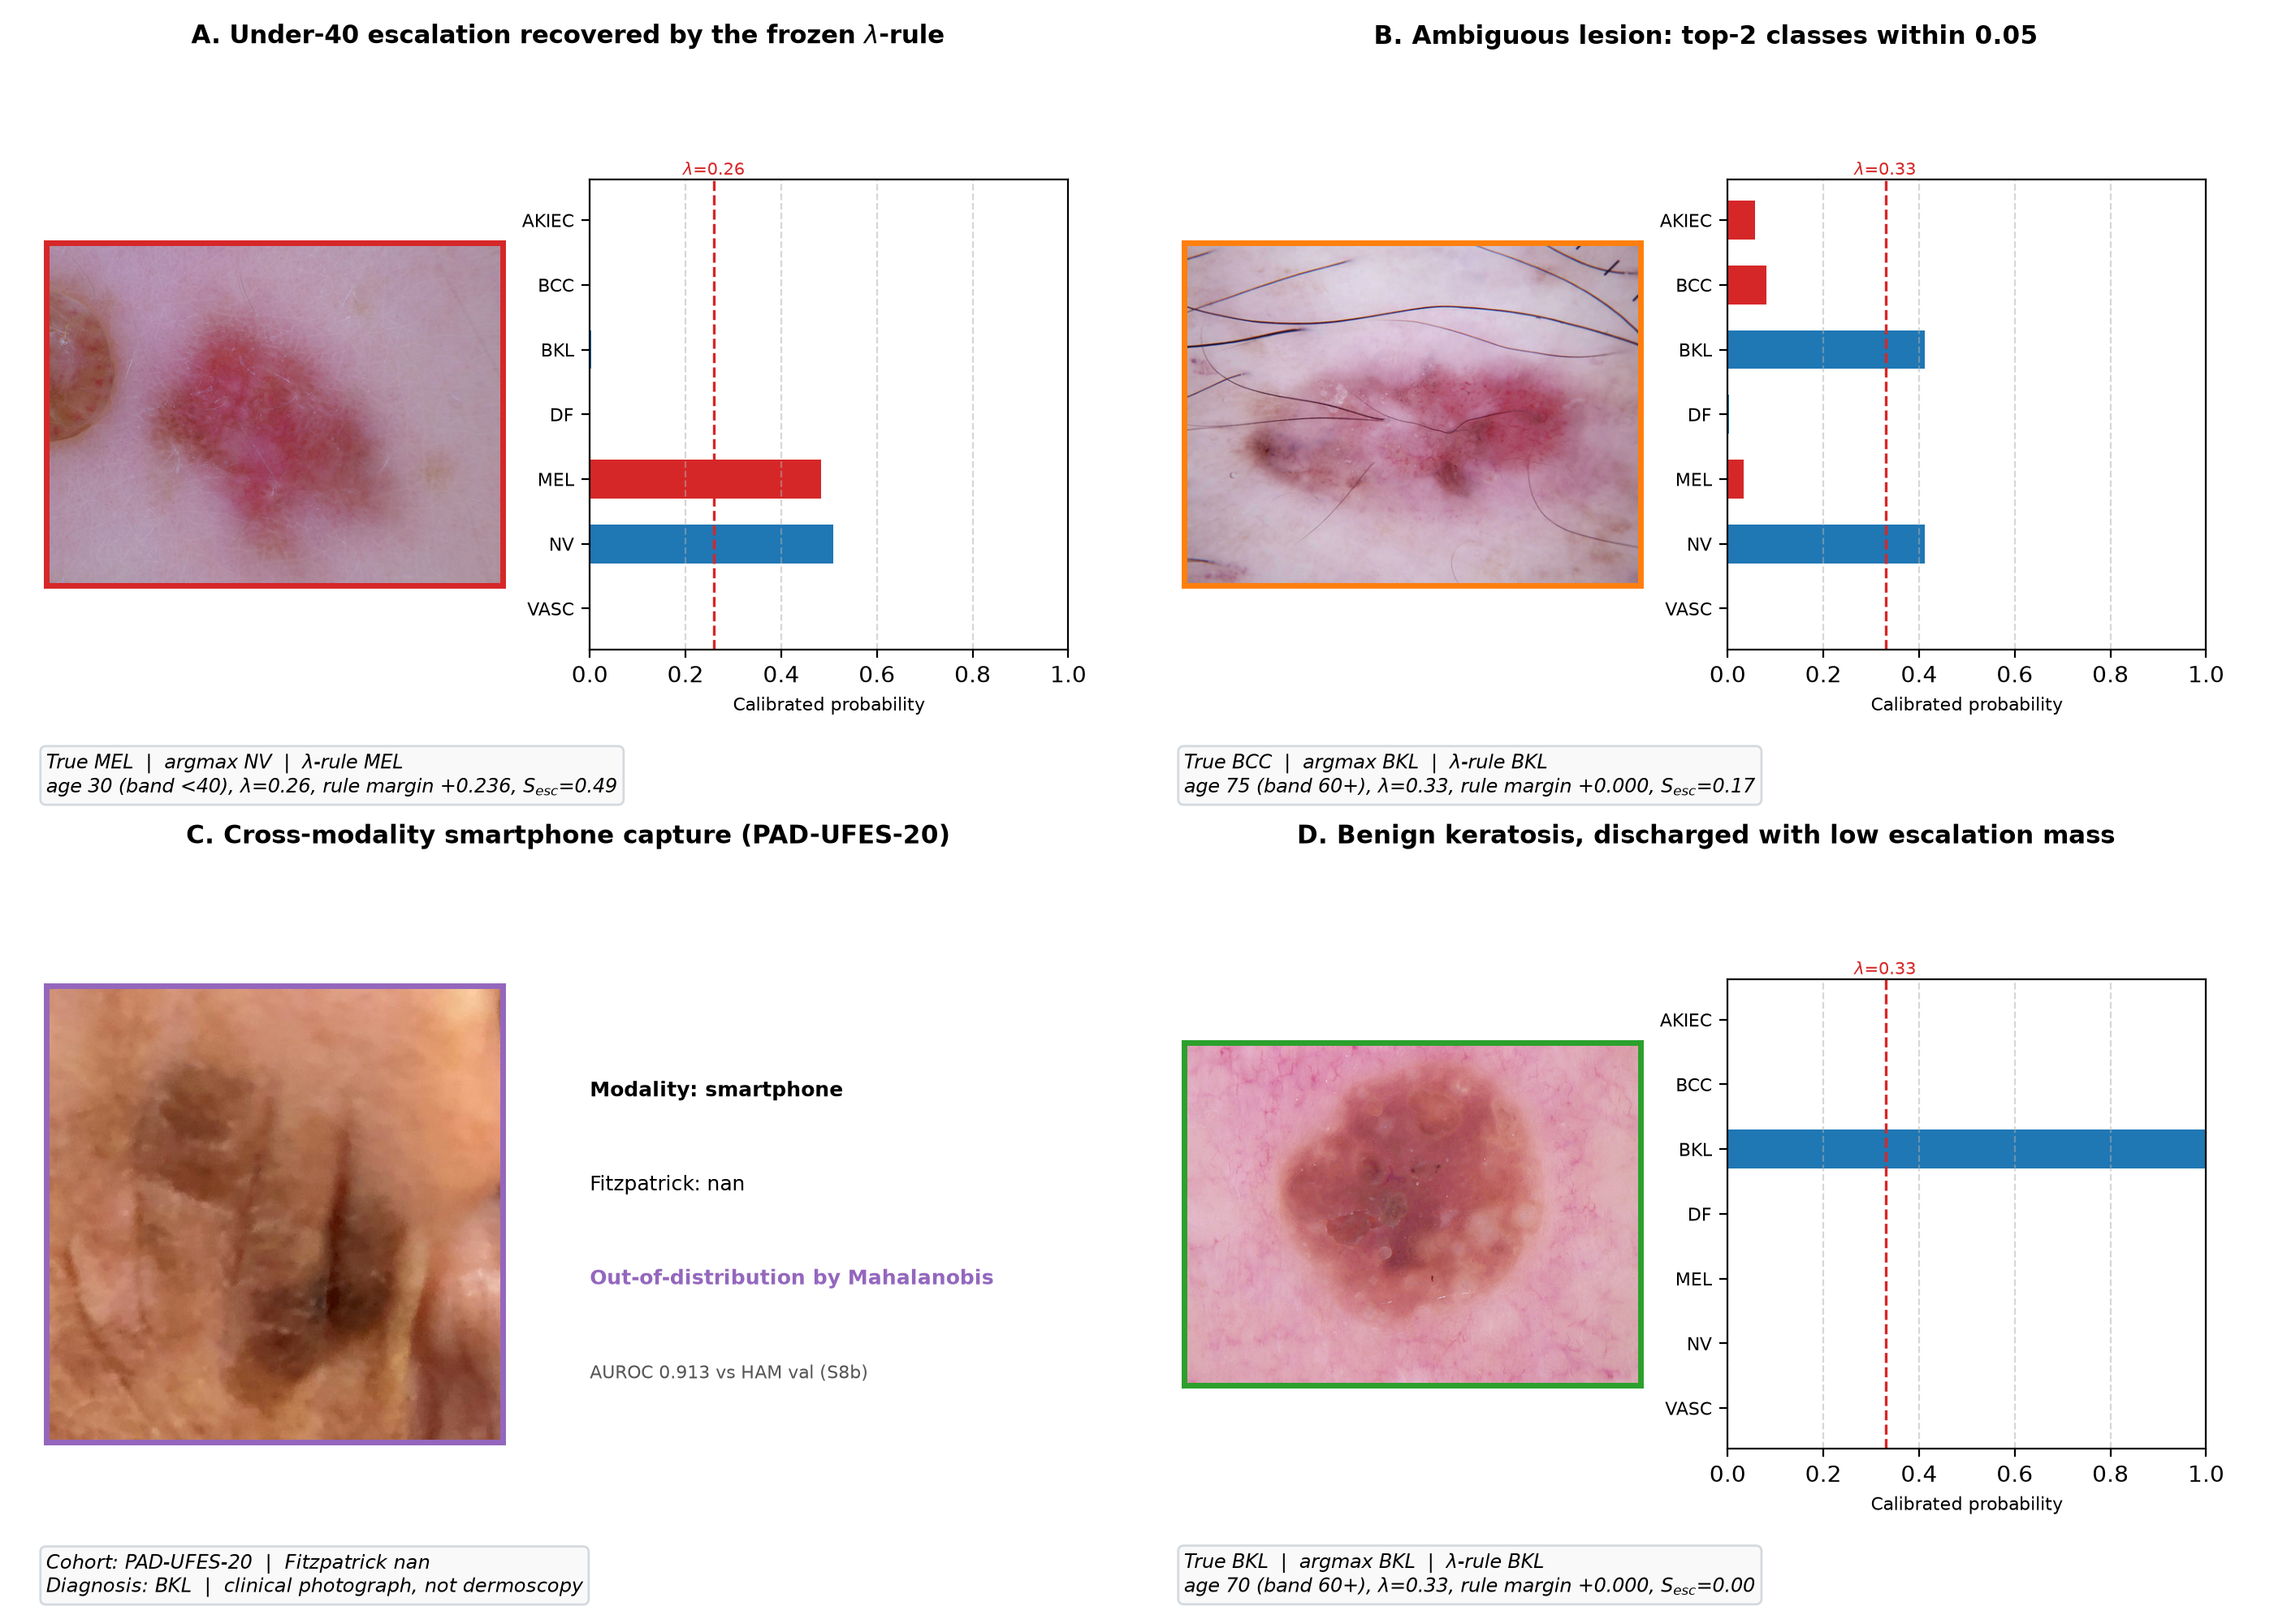
\includegraphics[width=\textwidth]{external_figure_case_atlas.png}
\caption{Exemplar lesions whose predicted class changes under the frozen age-conditional
rule. Panels are selected by \emph{running} the rule and taking the cases whose argmax label
was benign and whose rule label escalates, not by thresholding a score; a panel with no
qualifying case is rendered empty rather than relaxed. Across the out-of-fold panel the rule
rescues $205$ argmax misses, four of them melanomas in patients under $40$. This atlas is
qualitative support for the mechanism described in the main text and carries no claim of its
own.}
\label{fig:case_atlas}
\end{figure}

\end{document}
